\documentclass[a4paper]{article}

\usepackage[spanish]{babel}
	\selectlanguage{spanish}
\usepackage{geometry}
	\newgeometry{margin=3cm}
\usepackage{setspace}
\usepackage{graphicx}
\usepackage{float}
\usepackage[utf8]{inputenc}

\title{Reporte del Producto 6}
\author{Ana Gabriela Carretas Talamante}
\date{17 de abril de 2015}

\begin{document}
\maketitle
\section{Fuerza de arrastre}
Un objeto que cae a través de un gas o líquido experimenta una fuerza en sentido opuesto a su movimiento, esta está definida como la fuerza de arrastre, y se expresa como 
\begin{equation} 
\label{1}
F_D = \frac{\rho u^2 C_D A}{2}
\end{equation}

Puesto que el aire tiene viscosidad, existe una fuerza de arrastre de este tipo generada sobre la superficie de los cuerpos en movimiento, en ese medio. Para la realización de esta práctica se tomó en cuenta esta condición, y se pidió generar una comparación entre un tiro parabólico con condiciones ideales y uno considerando la fuerza de arrastre del aire.
\begin{figure}[H]
    \centering
    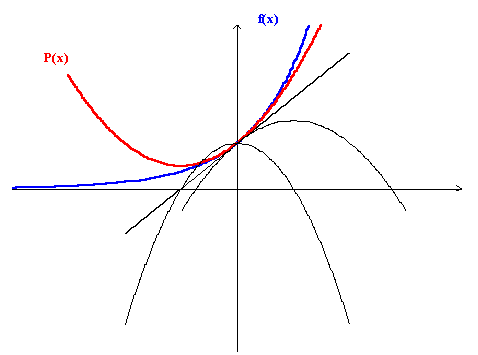
\includegraphics[width=12cm]{1}
  \end{figure} 

El número de Reynolds relaciona la densidad, viscosidad, velocidad y dimensión típica de un flujo en una expresión adimensional, que interviene en numerosos problemas de dinámica de fluidos. El caso más simple de flujo laminar a bajo número de Reynolds es el estudio del flujo alrededor de una esfera, ya realizado por G.G. Stokes en 1851. Y este caso en particular, de una esfera, es el que se utilizó para la realización de esta práctica.

  
\subsection{Ecuaciones de tiro parabólico considerando la resistencia del aire}
\label{uno}

Como estamos hablando de un tiro parabólico, sus ecuaciones permanecen iguales para las condiciones ideales, estas se mostraron a detalle en el producto 5. Para poder definir las ecuaciones modificadas por el efecto de la resistencia del aire, necesitamos definir ciertas constantes que dependen del proyectil. \\

\subsubsection{Consideraciones en el programa}

Para la práctica se utilizó como proyectil una esfera de radio $0.05 m$ y masa $0.25 kg$. El coeficiente de arrastre de una esfera es de $0.47$, y $\rho$, que representa la densidad del gas o fluido, a nivel del mar es de $1.29 \frac{kg}{m^3}$. \\

Para poder obtener las componentes de posición, velocidad y aceleración, en ambos ejes y por cada instante de tiempo, tendríamos que hacer hasta lo imposible si se pretende realizar de manera manual, por ello, se recurrió a utilizar en el algoritmo un ciclo que se hiciera cargo de estas cuentas. \\

Como valores de entrada, tenemos que piden como datos iniciales a $ag, v_o, x_o, y_o$. Siendo $ag$ el ángulo inicial medido en grados, $v_o$ la velocidad inicial en $\frac{m}{s}$ y $x_o, y_o$ como las componentes iniciales en su eje respectivo.\\

Se crearon dos subrutinas, una que se dedicara al cálculo sin fricción, y la otra al cálculo con fricción.En cada una se ingresaban los mismos datos iniciales, y arrojaban $x_max, y_max, t_f$, siendo estos valores el desplazamiento máximo, la mayor altura y el tiempo total del lanzamiento, respectivamente. Además, en el programa se calculan los errores porcentuales entre ambos lanzamientos. \\

También se muestran las gráficas realizadas en \texttt{gnuplot} para comprobar el funcionamiento del programa y observar gráficamente las diferencias entre ambos tiros.

\section{Simulando un tiro parabólico}
Se presentará a continuación el código modificado del producto 5, agregándole el cálculo de un tiro parabólico considerando la resistencia del aire y comparaciones entre ambos lanzamientos.
  \subsection{Código en \texttt{Fortran}}
\begin{verbatim}
!************************************************  
!This program plots projectile motion of an object.  
!The program requires user input for initial velocity   
!and angle of the object.The algorithm uses a time   
!step of 0.01 second i.e. it calculates object's  
!location in the x and y plane every 0.01 second.  
!**********By: Waleed Ishaque, 2013**************

!Modificaciones para el curso de Programacion en FORTRAN
!Universidad de Sonora, Gabriela Carretas, 2015.

module constantes
implicit none
  real, parameter :: pi = 4.0*atan(1.0)
  real, parameter :: g = 9.80
  real, parameter :: ar = (4.0*atan(1.0))/180 
  real, parameter :: c = 0.47
  real, parameter :: ro = 1.29
  real, parameter :: rad = 0.05
  real, parameter :: m = 0.25
  integer, parameter :: npts = 5000

  !g es la gravedad, pi es "pi"
  !ar es para convertir grados a radianes
  !c es el coeficiente de arrastre de una esfera
  !ro es la densidad del aire a nivel del mar
  !rad es el radio de la esfera
  !m es la masa del proyectil
  !npts es la cantidad de puntos que graficara el programa

end module constantes

!---------------------------------------
!Subrutina 1
subroutine sinfriccion (ag, vo, xo, yo, rs, hs, ts)
  use constantes
  implicit none
  integer :: i
  real :: ag, vo, xo, yo, rs, hs, ts
  real, dimension (0:npts) :: vx, vy, x, y, t  
  !--------------------------------------
  !vo es la velocidad inicial del objeto   
  !ag es el angulo inicial del objeto
  !xo, yo son la posición inicial del objeto
 
  !ts es el tiempo total de vuelo
  !rs es la distancia maxima de x
  !hs es la altura maxima que alcanza el proyectil

  !vx, vy son contadores de las componentes de velocidad respectivas
  !x,y son contadores de las componentes de posición respectivas
  !i es un contador
  !-------------------------------------

  !Para convertir el angulo a radianes   
  ag = ag*ar

  !Las componentes de velocidades
  vx(0) = vo*cos(ag)
  vy(0) = vo*sin(ag)

  !Comenzaremos a graficar con este algoritmo   
  open(1, file='sinfriccion.dat')   
  do i=1, npts, 1

      !Calculamos el instante
     t(i) = float(i)*0.01 
     
     !Calculamos la posicion para cada instante     
     x(i) = xo+vx(0)*t(i)   
     y(i) = yo+vy(0)*t(i) - 0.5*g*t(i)*t(i)   

     !Escribimos los resultados en el algoritmo graficador   
     write(1,1001) x(i), y(i)
     1001 format (f11.5, f11.5)

     !El programa termina cuando vuelve al suelo   
     if (y(i)<0) exit   
  end do
  close(1)

  !Calculamos el tiempo total de vuelo
  ts = (2*vy(0))/g

  !Calculamos la altura maxima del proyectil
  hs = yo+((vy(0)*vy(0))/(2*g))

  !Calculamos la distancia maxima condicionada
  if (ag<=0) then
     rs = 0
  else if (ag==(pi/2)) then
     rs = 0
  else
     rs = xo+vx(0)*ts
  endif
end subroutine sinfriccion
    
!---------------------------------------
!Subrutina 2
subroutine confriccion (ag, vo, A, d, xo, yo, tf, hf, rf)    
  use constantes
  implicit none
  integer :: ii
  real :: ag, vo, A, d, xo, yo, tf, hf, rf
  real, dimension (0:npts) :: vxx, vyy, ax, ay, xx, yy, tt
  !----------------------
  !A es el area del proyectil, en este caso, una esfera
  !d es la densidad de la esfera con respecto al aire
  !tf es el tiempo total de vuelo con friccion
  !hf es la altura maxima que alcanza el proyectil con friccion  
  !rf es la distancia maxima de x con friccion
  
  !ax, ay son contadores de las componentes de velocidad respectivas con friccion
  !vxx, vyy son contadores de las componentes de velocidad respectivas con friccion  
  !xx,yy son contadores de las componentes de posicion respectivas con friccion
  !ii es un contador
  !----------------------

  !Para el area del proyectil
  A = rad*rad*pi
  
  !Para la densidad del proyectil
  d = (ro*c*A*0.5)

  !Las componentes de posicion iniciales
  xx(0) = xo
  yy(0) = yo

  !Las componentes de velocidad iniciales
  vxx(0) = vo*cos(ag)
  vyy(0) = vo*sin(ag)
  
  !Las componentes de aceleración iniciales
  ax(0) = -(d/m)*vxx(0)*vxx(0)
  ay(0) = -(g)-((d/m)*vyy(0)*vyy(0))

  !Tiempo inicial
  tt(0) = 0

  !Comenzaremos a graficar con este algoritmo   
  open(2, file='friccion.dat')   
  !Escribiendo los valores inciales
  write (2,1001) xx(0), yy(0)
  1001 format (f11.5, f11.5)
  do ii = 0, npts, 1
     
     !Calculamos el instante
     tt(ii+1) = tt(ii)+0.01 
    
     !Calculamos las componentes de velocidad para cada instante 
     vxx(ii+1) = vxx(ii)+ax(ii)*tt(ii+1)   
     vyy(ii+1) = vyy(ii)+ay(ii)*tt(ii+1)  

     !Calculamos las componentes de aceleracion para cada instante
     ax(ii+1) = -(d/m)*vxx(ii)*vxx(ii)
     ay(ii+1) = -(g)-((d/m)*vyy(ii)*vyy(ii))

     !Calculamos la posicion para cada instante
     xx(ii+1) = xx(ii)+vxx(ii)*tt(ii+1)+(0.5*ax(ii)*tt(ii+1)*tt(ii+1))
     yy(ii+1) = yy(ii)+vyy(ii)*tt(ii+1)+(0.5*ay(ii)*tt(ii+1)*tt(ii+1))
     
     !Escribimos los resultados en el algoritmo graficador   
     write(2,1001) xx(ii+1), yy(ii+1)  

     !El programa termina cuando vuelve al suelo   
     if (yy(ii+1)<0) exit   
  end do
  close(2)

  !Calculamos el tiempo total de vuelo
  tf = tt(ii)*10.0

  !Calculamos la altura maxima del proyectil
  hf = maxval(yy)

  !Calculamos el desplazamiento maximo del proyectil
  rf = xx(ii)
end subroutine confriccion

!----------------------------------------------------     
program proyectil2
  use constantes
  implicit none
  real :: ag, vo, xo, yo, rs, hs, ts
  real, dimension (0:npts) :: vx, vy, x, y, t, vxx, vyy, ax, ay, xx, yy, tt
  real :: A, d, tf, hf, rf
  real :: ex, ey
  !ex es el error porcentual en x
  !ey es el error porcentual en y

  !El usuario debe proporcionar datos iniciales
  write (*,*) 'Programa comparativo entre tiros parabolicos con y sin friccion del aire'
  write (*,*) 'Se tiene en consideracion de proyectil a una esfera con las siguientes especificaciones:'
  write (*,*) 'Masa=0.25 kg y Radio=0.05 m'  
  write (*,*) '------------------------------------------------'  
  write (*,*) 'Ingrese el angulo del proyectil en grados (Real)'   
  read *, ag   
  write (*,*) 'Ingrese la posicion inicial x en metros (Real)'   
  read *, xo
  write (*,*) 'Ingrese la posicion inicial y en metros (Real)'   
  read *, yo
  write (*,*) 'Ingrese la velocidad del proyectil en m/s (Real)'   
  read *, vo  
  write (*,*) '------------------------------------------------'   
  !---------------------------------------
  call sinfriccion (ag, vo, xo, yo, rs, hs, ts)
  call confriccion (ag, vo, A, d, xo, yo, tf, hf, rf)

  !Para calcular el error porcentual del tiro sin friccion
  ex = ((rs-rf)/rf)*100
  ey = ((hs-hf)/hf)*100

  !Generamos los resultados para el usuario
  write (*,*) 'Para un proyectil con velocidad inicial=',vo,'m/s y un angulo=',ag,'radianes'
  write (*,*) '------------------------------------------------'  
  write (*,*) 'Resultados en el tiro sin friccion:'
  write (*,*) 'Tiempo total de vuelo=',ts,'s'
  write (*,*) 'Altura maxima=',hs,'m'
  write (*,*) 'Distancia maxima=',rs,'m'
  write (*,*) '------------------------------------------------'  
  write (*,*) 'Resultados en el tiro con friccion:'
  write (*,*) 'Tiempo total de vuelo=',tf,'s'
  write (*,*) 'Altura maxima=',hf,'m'
  write (*,*) 'Distancia maxima=',rf,'m'
  write (*,*) '------------------------------------------------'  
  write (*,*) 'La diferencia en x entre ambos casos es=',ex,'%'
  write (*,*) 'La diferencia en y entre ambos casos es=',ey,'%'
  !cerramos el programa   
end program proyectil2

\end{verbatim}

Ahora, hacemos énfasis en el código que se encarga de guardar los datos arrojados por el programa cada centésima de segundo, en 6,000 ocasiones. Este se encarga de crear un archivo \texttt{.dat} en ambos casas, con los cuales próximamente graficaremos en el programa \texttt{gnuplot} desde la terminal.

\subsubsection{Código para graficar en "sinfriccion"}
\begin{verbatim}
  !Comenzaremos a graficar con este algoritmo   
  open(1, file='sinfriccion.dat')   
  do i=1, npts, 1

      !Calculamos el instante
     t(i) = float(i)*0.01 
     
     !Calculamos la posicion para cada instante     
     x(i) = xo+vx(0)*t(i)   
     y(i) = yo+vy(0)*t(i) - 0.5*g*t(i)*t(i)   

     !Escribimos los resultados en el algoritmo graficador   
     write(1,1001) x(i), y(i)
     1001 format (f11.5, f11.5)

     !El programa termina cuando vuelve al suelo   
     if (y(i)<0) exit   
  end do
  close(1)
\end{verbatim}  

\subsubsection{Código para graficar en "confriccion"}
La diferencia con el código anterior es que, para cada instante de tiempo cambian las componentes de velocidad, y por ende, las de aceleración. Se vuelven valores temporales los de tiempo, velocidad, aceleración y posición, al final se registran sólo los de posición en la hoja de datos.
\begin{verbatim}
  !Comenzaremos a graficar con este algoritmo   
  open(2, file='friccion.dat')   
  !Escribiendo los valores inciales
  write (2,1001) xx(0), yy(0)
  1001 format (f11.5, f11.5)
  do ii = 0, npts, 1
     
     !Calculamos el instante
     tt(ii+1) = tt(ii)+0.01 
    
     !Calculamos las componentes de velocidad para cada instante 
     vxx(ii+1) = vxx(ii)+ax(ii)*tt(ii+1)   
     vyy(ii+1) = vyy(ii)+ay(ii)*tt(ii+1)  

     !Calculamos las componentes de aceleracion para cada instante
     ax(ii+1) = -(d/m)*vxx(ii)*vxx(ii)
     ay(ii+1) = -(g)-((d/m)*vyy(ii)*vyy(ii))

     !Calculamos la posicion para cada instante
     xx(ii+1) = xx(ii)+vxx(ii)*tt(ii+1)+(0.5*ax(ii)*tt(ii+1)*tt(ii+1))
     yy(ii+1) = yy(ii)+vyy(ii)*tt(ii+1)+(0.5*ay(ii)*tt(ii+1)*tt(ii+1))
     
     !Escribimos los resultados en el algoritmo graficador   
     write(2,1001) xx(ii+1), yy(ii+1)  

     !El programa termina cuando vuelve al suelo   
     if (yy(ii+1)<0) exit   
  end do
  close(2)
\end{verbatim} 

Ahora se muestra el código utilizado en \texttt{gnuplot} desde la terminal para poder graficar en las diferentes ocasiones de ángulo que se ingresaron. \\
\begin{verbatim}set title "Tiro con angulo de -- grados, xo= -- m, yo = -- m y vo= -- m/s" 
set xlabel "Distancia"
set ylabel "Altura"
set grid
plot "sinfriccion.dat", "friccion.dat"
\end{verbatim}

\subsection{Corriendo el programa}
\label{dos}

\subsubsection{Ángulo de 30 grados}
\begin{figure}[H]
    \centering
    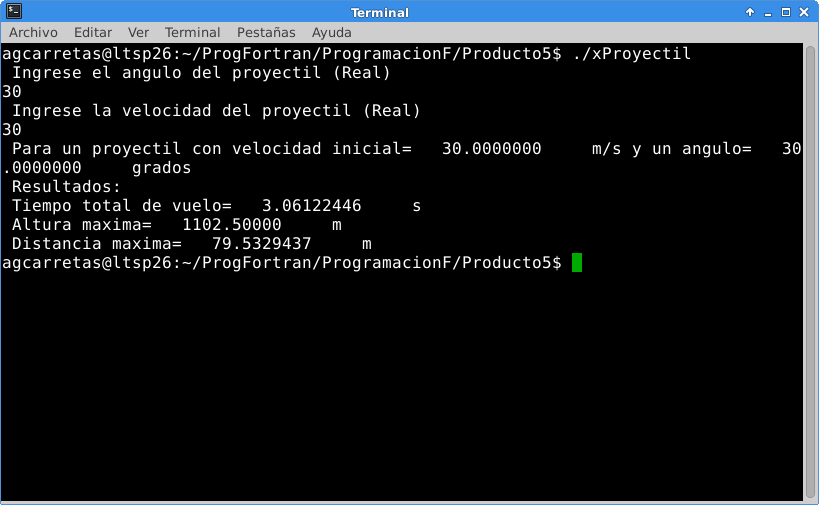
\includegraphics[width=12cm]{30} \\
    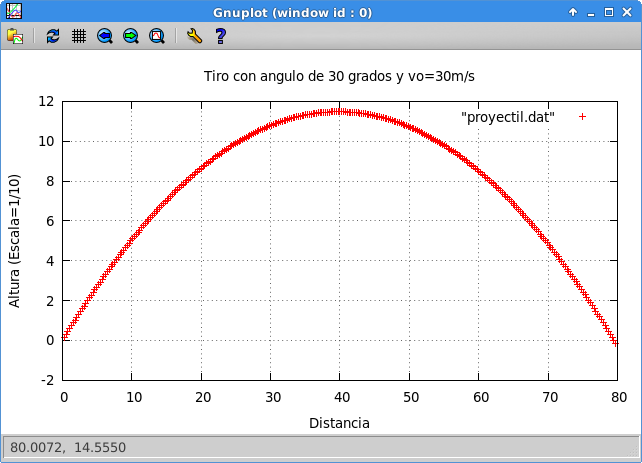
\includegraphics[width=12cm]{30plot}
  \end{figure} 

\subsubsection{Ángulo de 45 grados}
\begin{figure}[H]
    \centering
    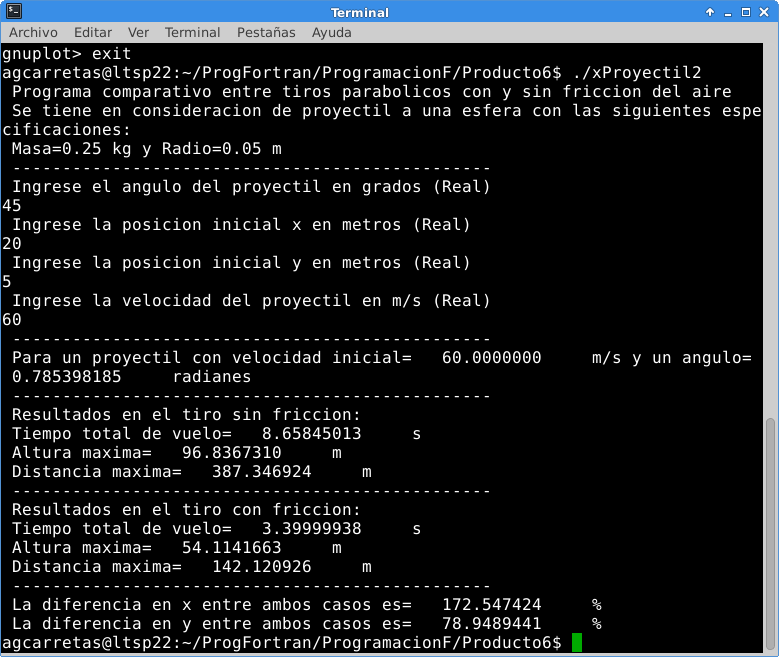
\includegraphics[width=12cm]{45} \\
    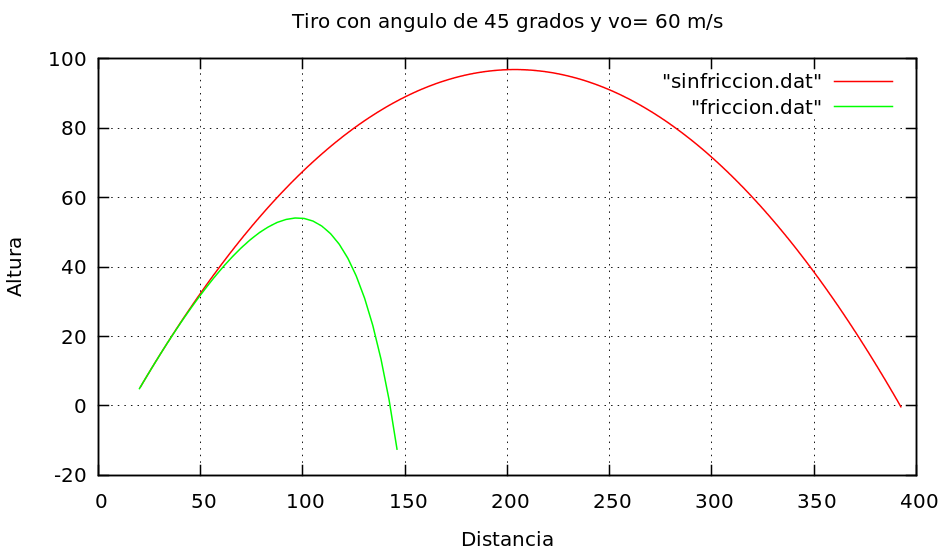
\includegraphics[width=12cm]{45plot}
  \end{figure} 

\subsubsection{Ángulo de 60 grados}
\begin{figure}[H]
    \centering
    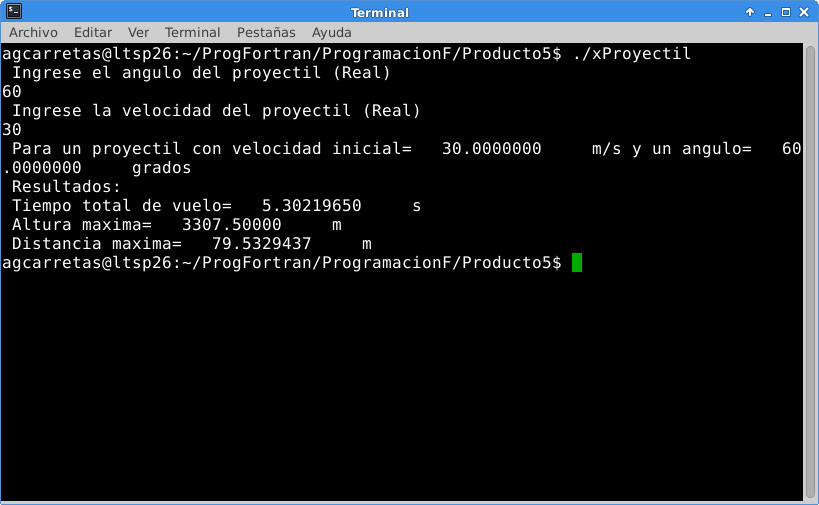
\includegraphics[width=12cm]{60} \\
    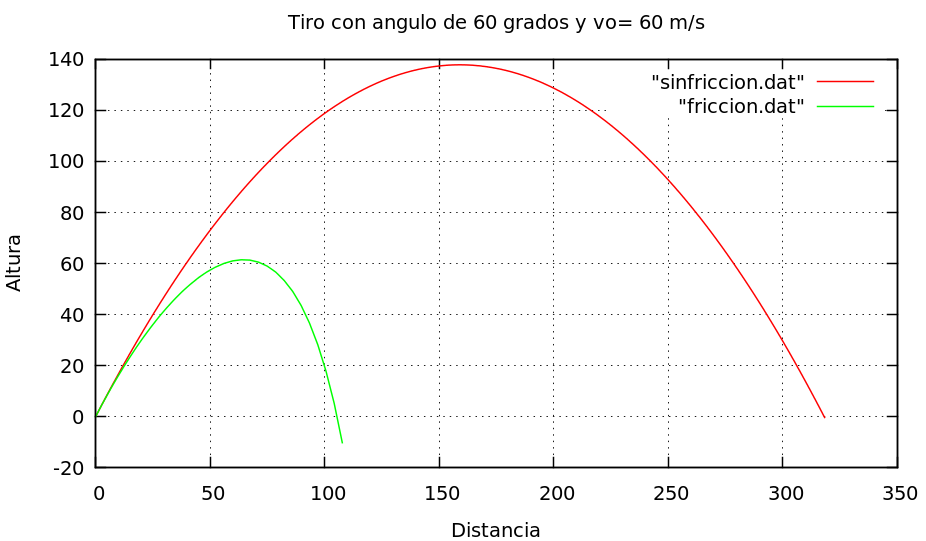
\includegraphics[width=12cm]{60plot}
  \end{figure} 

\end{document}
